% ============================================================
%  Appendix A: Evaluation details
% ============================================================
\chapter{Evaluation Details}
\label{app:eval}

This appendix collects protocol details of \chapref{ch:experiments} that matter for
reproducing the numbers but not for reading the results.

\section[Which Published Table Each Benchmark Cites]{Which Published Table Each\newline Benchmark Cites}
The published comparison point differs per benchmark, chosen so that the cited
protocol matches ours exactly rather than the nearest available number.
MAW cites CD-IID Table~1: both the MAW authors' own evaluation code and our
local harness apply the identical scaling and metrics.
ARAP cites Ordinal Shading Table~1, \emph{not} CD-IID Table~2: CD-IID modifies
the ARAP scene set (dropping redundant illuminations and adding scenes from the
MIST dataset), a set we cannot reproduce, whereas Ordinal Shading's table uses
the original Bonneel et al.\ scenes (the same 52-scene set used throughout
this chapter). IIW cites Ordinal Shading Table~2 for its zero-shot WHDR figure,
alongside the fuller reproduced roster of \mycite{yuan25texture}.
MID has no external citation on any axis; it is a ground-truth-free constancy
metric that no other published work reports, and MIDIntrinsics is training data
for both this model and CD-IID, which additionally disqualifies it as a
zero-shot benchmark for either.

\section{Inference Resolution}
Inference resolution is fixed per benchmark rather than shared uniformly.
MID, IIW, and ARAP use an aspect-preserving maximum side length of 1280 pixels;
measured directly on the full ARAP set, 1280 and 1500 pixels give effectively
identical scores (every metric moves by less than 1\%, in mixed directions,
consistent with measurement noise rather than a real effect), so 1280 is kept
throughout for consistency and lower memory use.
Ordinal Shading \mycite{careaga23ordinal} instead resizes each ARAP image to a
content-adaptive resolution $R_0$ (Miangoleh et al.'s edge-density criterion),
capped at 1500 pixels; since $R_0$ is computed per image and not reproducible
from the published protocol alone, no fixed resolution can replicate it exactly,
and the 1280-vs-1500 measurement above shows that choice is immaterial to our
own scores regardless.
MAW also uses the common 1280-pixel inference cap. Its public scorer then
resizes every prediction and region mask to $320\times240$ before computing the
metrics, so the reported numbers are determined at that fixed scoring scale.
Every locally run method, including the baselines, is evaluated at the same
resolution within each benchmark.
\figref{fig:maw_resolution} shows the qualitative plateau this is chosen from:
raising the full-CIAI prediction from 1280 to 1792 or 2560 changes little
visually, whereas 512 visibly softens fine structure at the resolutions where
that matters (MID, IIW).

\begin{figure}[t!]
  \centering
  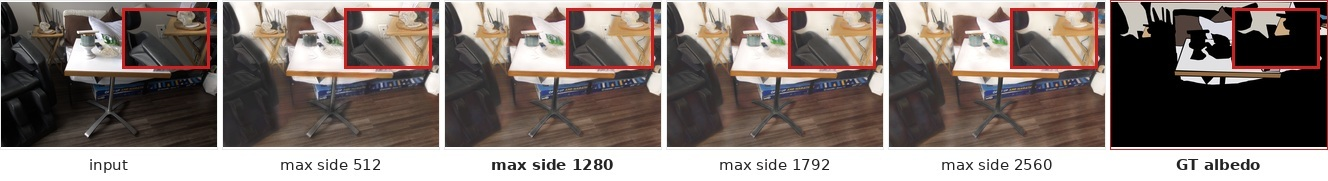
\includegraphics[width=\textwidth]{images/hires/maw_resolution.jpg}
  \caption[Inference-resolution comparison on MAW.]{%
    Effect of inference resolution on a MAW scene with our model
    (\secref{sec:exp_setup}).
    The input photograph is shown on the left and the measured albedo on the
    right; the middle columns show predictions at different maximum side lengths.
    Each panel repeats the same black-sofa-armrest crop in the upper right with a red
    border to make blur differences easier to compare.
    Fine structure improves substantially from 512 to 1280 pixels, then largely
    plateaus. We therefore use the common 1280-pixel inference cap for every
    locally run MAW method; the official scorer subsequently reduces predictions
    to $320\times240$ before measuring the metrics.
  }
  \label{fig:maw_resolution}
\end{figure}

